\documentclass[12pt]{report}

\usepackage{style}
\bibliography{references.bib}
%\includeonly{chapter/chapter1} % use this to compile only the chapter you are currently working on

\begin{document}

%%%%%%%%%%%%%%%%%%%%%%%%%%%%%%%%%%%%%%%%%%%%%%%%%%%%%%%%%%
% # Title page
%%%%%%%%%%%%%%%%%%%%%%%%%%%%%%%%%%%%%%%%%%%%%%%%%%%%%%%%%%

\pagenumbering{gobble}
\centering
\vspace{3cm}

\doublespacing
THE PROCESSING AND ACCEPTABILITY OF GAPPED VS. RESUMPTIVE \\
RELATIVE CLAUSES IN FIRST AND SECOND LANGUAGE ENGLISH

\vspace{1.5cm}
\singlespacing
A DISSERTATION SUBMITTED TO THE GRADUATE DIVISION OF \\
THE UNIVERSITY OF HAWAI`I AT MĀNOA IN PARTIAL FULFILLMENT OF \\
THE REQUIREMENTS FOR THE DEGREE OF

\vspace{1cm}
\doublespacing
DOCTOR OF PHILOSOPHY \\
IN \\
SECOND LANGUAGE STUDIES

\vspace{1.5cm}
\singlespacing
MAY 2024

\vspace{1.5cm}
\doublespacing
By \\
Fred Zenker

\vspace{1.5 cm}
\singlespacing
Dissertation Committee: \\
Bonnie D. Schwartz, Chairperson \\
Kamil Deen \\
Li `Julie' Jiang \\
William O'Grady \\
Amy Schafer

\vspace*{\fill}
\flushleft
Keywords: relative clause, resumption, resumptive pronoun, adult second language acquisition, adult second language processing

\newpage

\pagenumbering{roman}
\setcounter{page}{1}
\vspace*{\fill}
\begin{centering}

Copyright \textcopyright \space 2024

\vspace{0.5 cm}

Fred Zenker

All Rights Reserved

\end{centering}

%%%%%%%%%%%%%%%%%%%%%%%%%%%%%%%%%%%%%%%%%%%%%%%%%%%%%%%%%%
% # Acknowledgments
%%%%%%%%%%%%%%%%%%%%%%%%%%%%%%%%%%%%%%%%%%%%%%%%%%%%%%%%%%

\chapter*{Acknowledgments}
\addcontentsline{toc}{chapter}{Acknowledgments}
\setlength{\parindent}{2.6em}
\setstretch{1.5}

Some text

%%%%%%%%%%%%%%%%%%%%%%%%%%%%%%%%%%%%%%%%%%%%%%%%%%%%%%%%%%
% # Abstract
%%%%%%%%%%%%%%%%%%%%%%%%%%%%%%%%%%%%%%%%%%%%%%%%%%%%%%%%%%

\chapter*{Abstract}
\addcontentsline{toc}{chapter}{Abstract}

Some text

\newpage

%%%%%%%%%%%%%%%%%%%%%%%%%%%%%%%%%%%%%%%%%%%%%%%%%%%%%%%%%%
% # Table of Contents
%%%%%%%%%%%%%%%%%%%%%%%%%%%%%%%%%%%%%%%%%%%%%%%%%%%%%%%%%%

\setstretch{1}
\renewcommand{\contentsname}{\vspace{-27pt} \begin{center} \normalsize \textbf{TABLE OF CONTENTS} \end{center} \vspace{-1.5cm}}
\renewcommand\thepage{\romannumeral\numexpr\value{page}\relax}
\phantomsection
\addcontentsline{toc}{chapter}{Table of Contents}
\tableofcontents
\newpage

%%%%%%%%%%%%%%%%%%%%%%%%%%%%%%%%%%%%%%%%%%%%%%%%%%%%%%%%%%
% # List of Tables
%%%%%%%%%%%%%%%%%%%%%%%%%%%%%%%%%%%%%%%%%%%%%%%%%%%%%%%%%%

\renewcommand{\listtablename}{\vspace{-80pt} \begin{center} \normalsize \textbf{LIST OF TABLES} \end{center} \vspace{-1.5cm}}
\phantomsection
\listoftables
\addcontentsline{toc}{chapter}{List of Tables}
\newpage

%%%%%%%%%%%%%%%%%%%%%%%%%%%%%%%%%%%%%%%%%%%%%%%%%%%%%%%%%%
% # List of Figures
%%%%%%%%%%%%%%%%%%%%%%%%%%%%%%%%%%%%%%%%%%%%%%%%%%%%%%%%%%

\renewcommand{\listfigurename}{\vspace{-77pt} \begin{center} \normalsize \textbf{LIST OF FIGURES} \end{center} \vspace{-1.5cm}}
\phantomsection
\listoffigures
\addcontentsline{toc}{chapter}{List of Figures}

%%%%%%%%%%%%%%%%%%%%%%%%%%%%%%%%%%%%%%%%%%%%%%%%%%%%%%%%%%
% # List of Abbreviations
%%%%%%%%%%%%%%%%%%%%%%%%%%%%%%%%%%%%%%%%%%%%%%%%%%%%%%%%%%

\chapter*{List of Abbreviations}
\addcontentsline{toc}{chapter}{List of Abbreviations}
\renewcommand\thepage{\romannumeral\numexpr\value{page}\relax}
\setstretch{1.5}

\noindent This dissertation makes use of the following abbreviations.

\begin{multicols}{2}
\begin{tabbing}
1 \hspace{1.5cm} \= 1st person \\
3 \> 3rd person \\
ACC \> Accusative \\
ADN \> Adnominal \\
AJT \> Acceptability judgment task \\
C \> Complementizer \\
\textit{CI} \> Confidence interval \\
CL \> Classifier \\
COMP \> Complementizer \\
CP \> Complementizer phrase \\
D \> Determiner \\
DEC \> Declarative \\
DET \> Determiner \\
DIST \> Distal demonstrative \\
DP \> Determiner phrase \\
EE \> ENS in the English AJT \\
ENS \> English native speaker \\
EPT \> Elicited production task \\
FEM \> Feminine \\
GEN \> Genitive \\
IL \> Interlanguage \\
INS \> Instrumental \\
KE \> KLE in the English AJT \\
KK \> KLE in the Korean AJT \\
KLE \> L1-Korean L2er of English \\
L1 \> First language \\
L2 \> Second language \\
L2er \> L2 learner \\
LOC \> Locative \\
M \> Masculine \\
MASC \> Masculine \\
ME \> MLE in the English AJT \\
MLE \> L1-Mandarin L2er of English \\
MM \> MLE in the Mandarin AJT \\
$n$ \> Sample size \\
N \> Noun \\
NOM \> Nominative \\
NP \> Noun phrase \\
ORC \> Direct object relative clause \\
$p$ \> $p$-value \\
PL \> Plural \\
PRED \> Predicate position \\
PRES \> Present \\
PROX \> Proximal demonstrative \\
PST \> Past \\
RC \> Relative clause \\
REL \> Relativizer \\
RP \> Resumptive pronoun \\
S \> Singular \\
\textit{SD} \> Standard deviation \\
\textit{SE} \> Standard error \\
SG \> Singular \\
SPRT \> Self-paced reading task \\
SRC \> Subject relative clause \\
T \> Tense \\
$t$ \> $t$-statistic \\
TL \> Target language \\
TOP \> Topic \\
TP \> Tense phrase \\
V \> Verb \\
VP \> Verb phrase \\
WH \>\textit{Wh}-feature \\
$z$ \> $z$-statistic \\
$\alpha$ \> First-argument position \\
$\beta$ \> Second-argument position \\
$\hat{\beta}$ \> Parameter estimate \\
\end{tabbing}
\end{multicols}

\noindent In linguistic examples with interlinear glossing, personal pronouns are represented with a number followed by one or more letters. For instance, ``1S'' marks a 1st person singular pronoun and ``3MS'' marks a 3rd person masculine singular pronoun. Complementizers are abbreviated to ``COMP'' in interlinear glosses and to ``C'' in syntactic trees. Hebrew Academy romanization is used to transcribe Hebrew sentences, Yale romanization is used to transcribe Korean sentences, and pinyin romanization is used to transcribe Mandarin sentences. Ungrammatical sentences are marked with asterisks.

\newpage

%%%%%%%%%%%%%%%%%%%%%%%%%%%%%%%%%%%%%%%%%%%%%%%%%%%%%%%%%%
% # Chapters
%%%%%%%%%%%%%%%%%%%%%%%%%%%%%%%%%%%%%%%%%%%%%%%%%%%%%%%%%%

\phantomsection
\renewcommand\thepage{\romannumeral\numexpr\value{page}\relax}
\pagenumbering{arabic}
\setcounter{page}{1}
\setstretch{1.5}
\setlength{\parskip}{0pt}

\addcontentsline{toc}{part}{Chapters}
\chapter{Title of First Chapter}

Some text (\cite{aarts2007}). Some text \textcite{aarts2007}; Some text Aarts (\citeyear{aarts2007}).

Take a look at Figure \ref{fig:sigmoid}.

\begin{figure}
\caption{Relationship between processing difficulty and helpfulness of resumption} \label{fig:sigmoid}
\raggedright\setstretch{1}
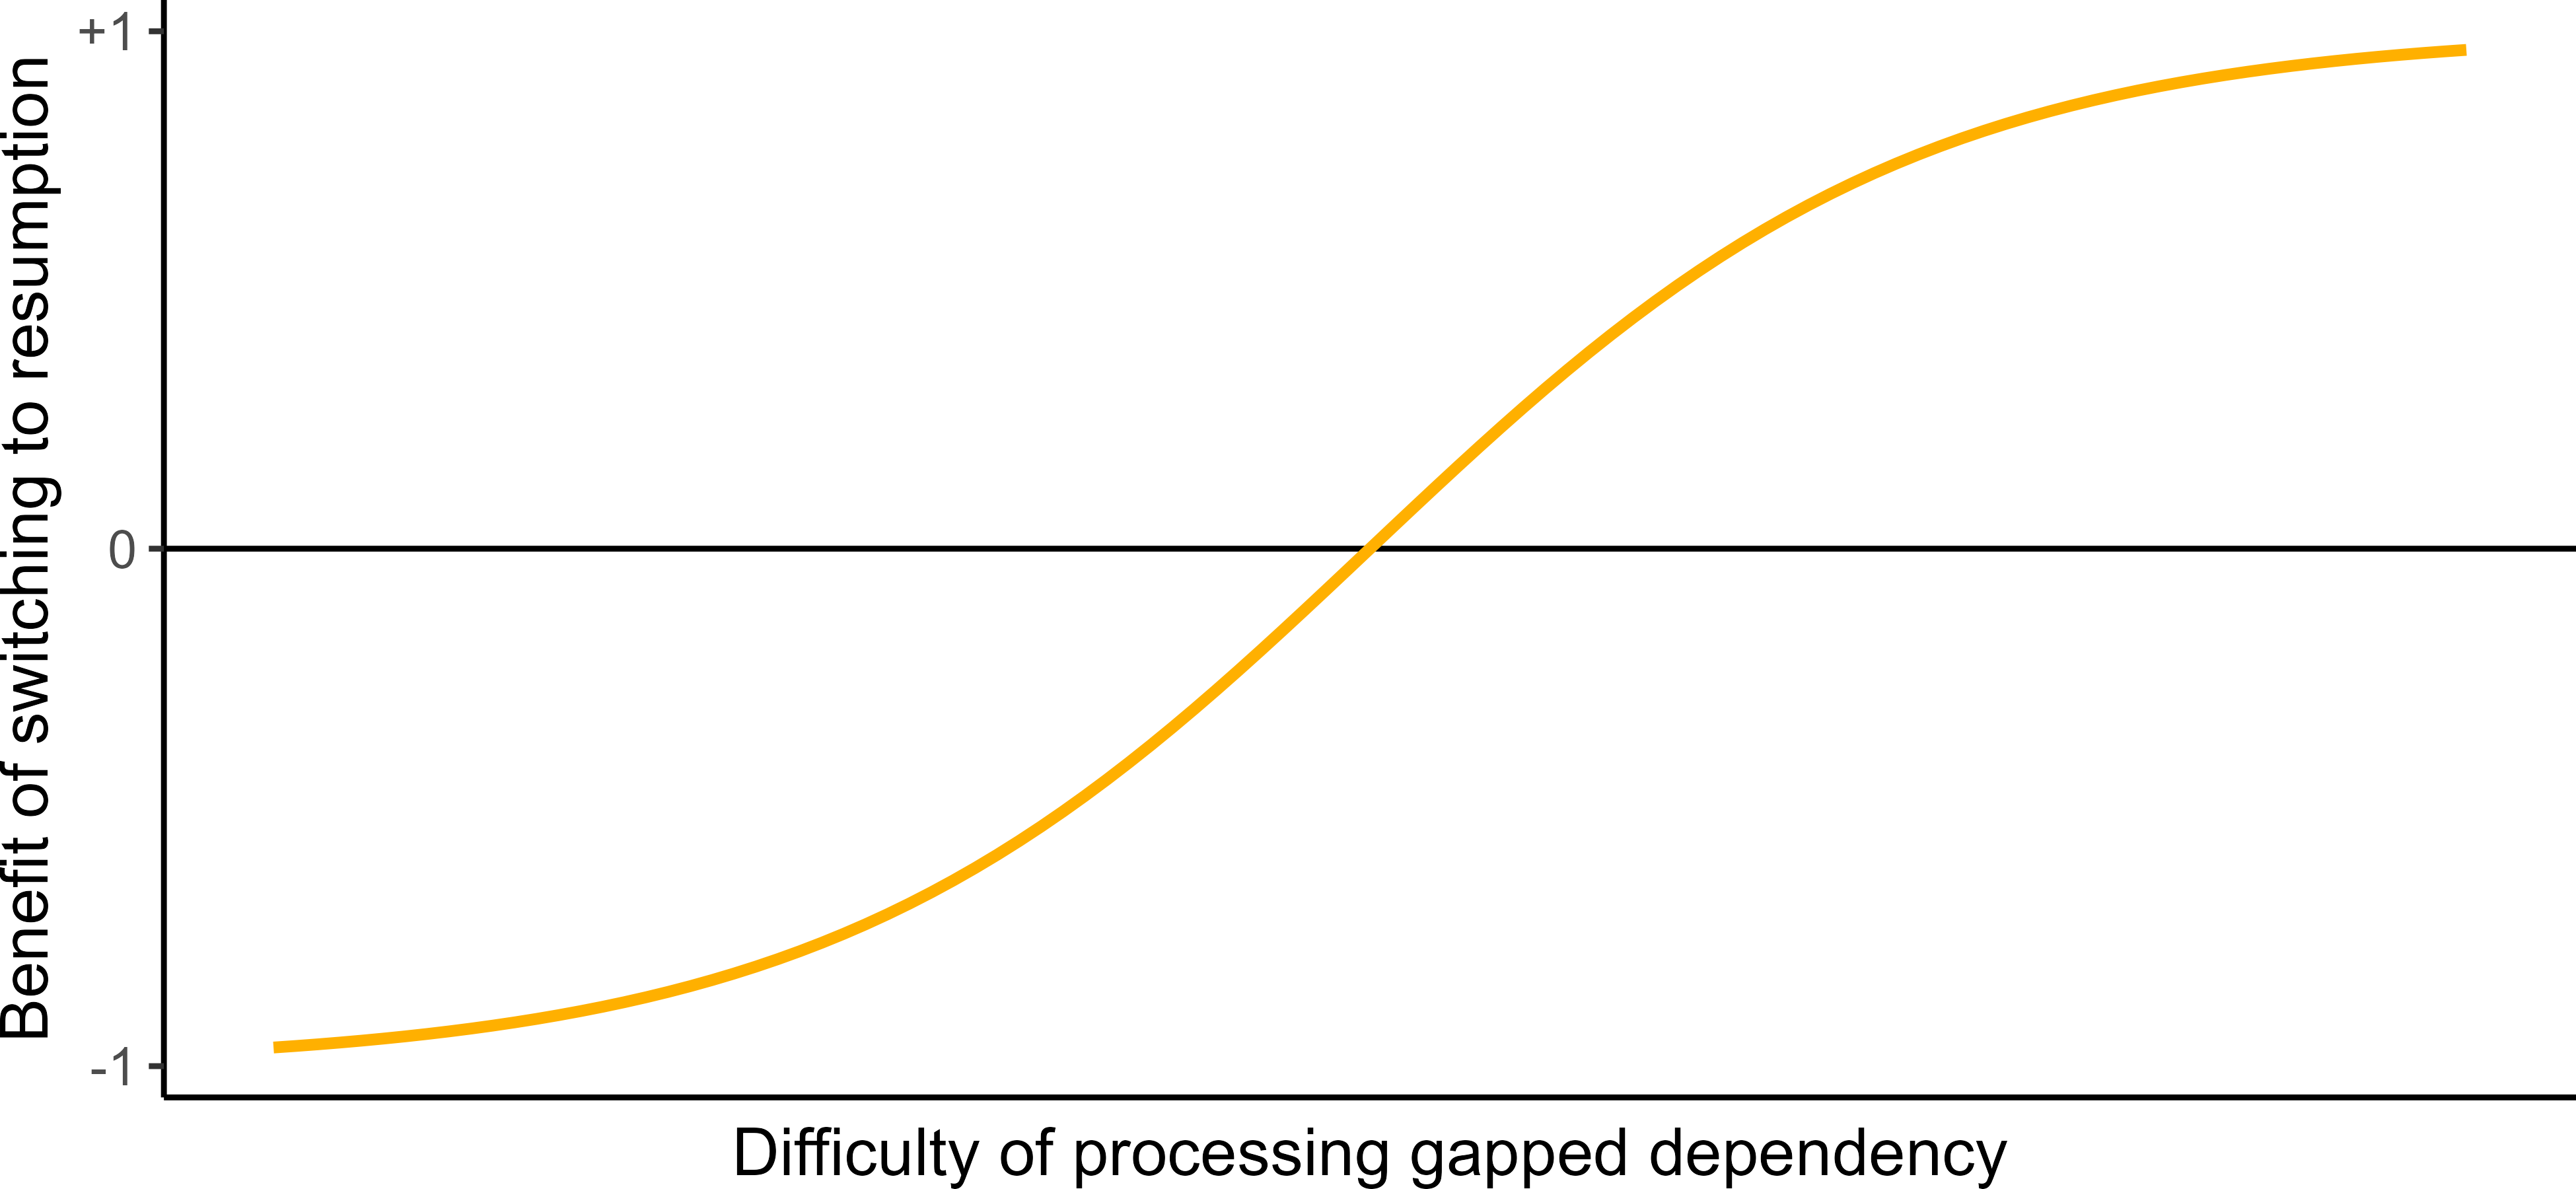
\includegraphics{image/sigmoid.png}
\vspace{-12pt}
\end{figure}

\noindent Some text.

\newpage

Of the four attempts at relativization shown below in Table \ref{tab:constraint}, the one in the [+Aboutness; +Sentential Category] cell (i.e.,~\textit{the dog that is fat}) is the only well-formed RC because it satisfies both the aboutness constraint and the sentential category constraint.

\begin{table}
\caption{Demonstration of the aboutness constraint and the sentential category constraint}\label{tab:constraint}
\raggedright\setstretch{1}
\begin{tabularx}{\linewidth}{XXX}\hline
& \phantom{* }+Aboutness & \phantom{* }−Aboutness\\\hline
+Sentential Category & \phantom{* }the dog [that is fat] & * the dog [that the cat is fat]\\
−Sentential Category & * the dog [that fat] & * the dog [that the cat]\\\hline
\end{tabularx}
\vspace{-12pt}
\end{table}

\noindent Some text.

\ex
people [who like dogs] \label{ex-horse}
\xe

\pex \label{ex-constraint}
\a Aboutness constraint: \par\nobreak\vspace{5pt} RCs are adjuncts and as such must provide supplementary information about their heads.
\a Sentential category constraint: \par\nobreak\vspace{5pt} RCs are sentential categories and as such must consist of at least one predicate and its core arguments, whose presence may be either overtly expressed or merely implied.
\xe

\pex[everygla=\ko] \label{ex-dog-ko}
\a
\begingl
\gla 뚱뚱한 개 //
\glb ttungttungha-n kay //
\glc fat-{\sc adn} dog //
\glft `the fat dog' / `the dog that is fat' //
\endgl \label{ex-dog-ko-1}
\a
\begingl
\gla 고양이를 좋아한 개 //
\glb koyangi-lul cohaha-n kay //
\glc cat-{\sc acc} like-{\sc adn} dog //
\glft `the dog that liked the cat' //
\endgl \label{ex-dog-ko-2}
\xe

\pex[everygla=\zh] \label{ex-dog-zh}
\a
\begingl
\gla 胖 的 狗 //
\glb pang de gou //
\glc fat {\sc adn} dog //
\glft `the fat dog' / `the dog that is fat' //
\endgl \label{ex-dog-zh-1}
\a
\begingl
\gla 喜歡 貓 的 狗 //
\glb xihuan mao de gou //
\glc like cat {\sc adn} dog //
\glft `the dog that likes the cat' //
\endgl \label{ex-dog-zh-2}
\xe
\chapter{Title of Second Chapter}

Some text

%%%%%%%%%%%%%%%%%%%%%%%%%%%%%%%%%%%%%%%%%%%%%%%%%%%%%%%%%%
% # Appendices
%%%%%%%%%%%%%%%%%%%%%%%%%%%%%%%%%%%%%%%%%%%%%%%%%%%%%%%%%%

\phantomsection
\setlength{\parindent}{0in}
\setstretch{1}

\appendix

\addcontentsline{toc}{part}{Appendices}
\chapter{Title of First Appendix}

Some text
\chapter{Title of Second Appendix}

Some text

%%%%%%%%%%%%%%%%%%%%%%%%%%%%%%%%%%%%%%%%%%%%%%%%%%%%%%%%%%
% # References
%%%%%%%%%%%%%%%%%%%%%%%%%%%%%%%%%%%%%%%%%%%%%%%%%%%%%%%%%%

\renewcommand{\bibname}{References}
\printbibliography
\addcontentsline{toc}{part}{References}

\end{document}